

 \documentclass[12t]{article}
 
 \usepackage[margin=1in]{geometry} 
 \usepackage{amsmath,amsthm,amssymb, mathtools}
 \usepackage{graphicx}
 \usepackage{subcaption}
 \usepackage{wrapfig}
 \usepackage{natbib}
 \bibliographystyle{plain}
 
 % Used to create code windows for Java
 \usepackage{listings}
 \usepackage{color}
 
 \definecolor{dkgreen}{rgb}{0,0.6,0}
 \definecolor{gray}{rgb}{0.5,0.5,0.5}
 \definecolor{mauve}{rgb}{0.58,0,0.82}
 
 \lstset{frame=tb,
 	language=Java,
 	aboveskip=3mm,
 	belowskip=3mm,
 	showstringspaces=false,
 	columns=flexible,
 	basicstyle={\small\ttfamily},
 	numbers=none,
 	numberstyle=\tiny\color{gray},
 	keywordstyle=\color{blue},
 	commentstyle=\color{dkgreen},
 	stringstyle=\color{mauve},
 	breaklines=true,
 	breakatwhitespace=true,
 	tabsize=3
 }

  
  \begin{document}
 	% PUT YOUR TITLE AND NAME HERE
 	\newcommand{\titlestr}{Mining Big Data - Map-Reduce}
 	\newcommand{\shorttitlestr}{Assignment 2}
 	\newcommand{\groupnames}{M. Vincent \& A. Phansalkar}
 	\newcommand{\studentids}{a1148120 \& a1776879}
 	\newcommand{\authorstr}{\groupnames}
 	
 	%%%%%%%%%%%%%%%%%%%%%%%%%%%%%%555
 	% title page
 	\begin{titlepage}
 		\centering
 		
 		{\LARGE \bf \titlestr \par}
 		\vspace{0.25cm}
 		{\large \bf \shorttitlestr \par}
 		
 		
 		\vspace{1cm}
 		{\large \authorstr \\}
 		{ \studentids \par}
 		\vspace{0.25cm}
 		
 		\large School of Computer Science, The University of Adelaide
 		
 		\vspace{1cm}
 		\today
 		
 		\vspace{3cm}
 		Report submitted for
 		{\bf COMP SCI 3306 Mining Big Data}
 		at the School of Computer Science,
 		University of Adelaide
 		
 		
\includegraphics[width=0.35\textwidth]{./Figures/UoA_logo_cmyk.pdf}
 		
 		\vspace{9cm}
 		

 	 	\vspace{1mm}
 		\noindent \hrulefill
 		
 		\vfill
 	\end{titlepage}
 	
 	\clearpage
 	\setcounter{page}{1}
	
	\section*{Exercise 1}

	The S-curves for each combination of $r$ and $b$ parameters have been calculated below. The threshold $t$ that defines how similar document need to be in order for be regarded as similar, can be approximated using the formula $t=(1/b)^{1/r}$. The threshold calculation has also been included below.
	
	These results were obtained by computing each of the formulae displayed below in the Excel workbook included in the assignment submission.  \\
	
	\begin{tabular}{cc}
	s & $1-(1-s^3)^{10}$ \\
	\hline
	0.1 & 0.010 \\
	0.2 & 0.077 \\
	0.3 & 0.239 \\
	0.4 & 0.484 \\
	0.5 & 0.737 \\
	0.6 & 0.912 \\
	0.7 & 0.985 \\
	0.8 & 0.999 \\
	0.9 & 1.000 \\
	\hline
	\end{tabular}
	\quad
	\begin{tabular}{cc}
	s & $1-(1-s^6)^{20}$ \\
	\hline
	0.1 & 0.000 \\
	0.2 & 0.001 \\
	0.3 & 0.014 \\
	0.4 & 0.079 \\
	0.5 & 0.270 \\
	0.6 & 0.615 \\
	0.7 & 0.918 \\
	0.8 & 0.998 \\
	0.9 & 1.000 \\
	\hline
	\end{tabular}
	\quad
	\begin{tabular}{cc}
	s & $1-(1-s^5)^{50}$ \\
	\hline
	0.1 & 0.000 \\
	0.2 & 0.016 \\
	0.3 & 0.115 \\
	0.4 & 0.402 \\
	0.5 & 0.796 \\
	0.6 & 0.983 \\
	0.7 & 1.000 \\
	0.8 & 1.000 \\
	0.9 & 1.000 \\
	\hline 
	\end{tabular} \\\\
	
	\begin{tabular}{ccc}
	r & b & t \\
	\hline
	3 & 10 & 0.464 \\
	6 & 60 & 0.607 \\
	5 & 50 & 0.457 \\
	\hline 
	\end{tabular} \\\\

	\begin{figure}[h]
	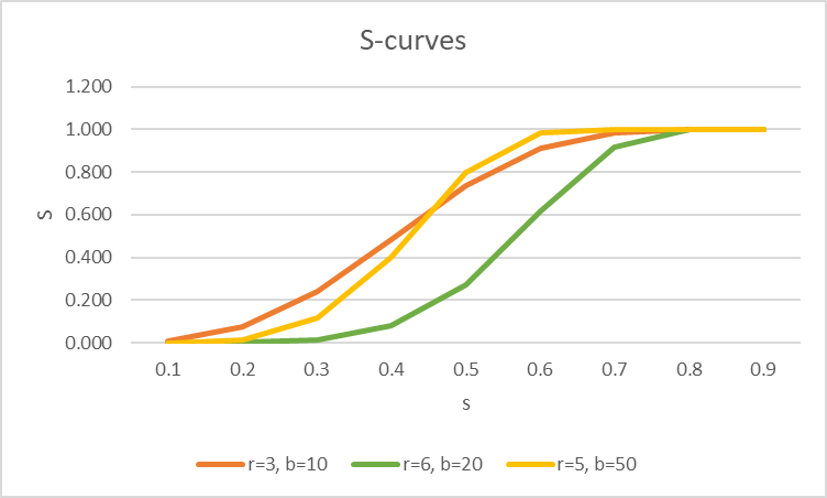
\includegraphics[width=0.8\textwidth]{./Figures/s-curves.png}\\	
	\caption{S-curves}
	\end{figure}

	\newpage
	
	\section*{Exercise 2}

	As noted in the text, the probability of a false positive is the probability of a 1 bit raised to the $k$th power, which is $(1-e^{-km/n})^k$. $k$ denotes the number of hash functions, $m$ is the number of  members in the set $S$, and $n$ is the number of bits in the array. 
	
	If there are 10 billion bits and 2 billion members of $S$, then $n=10$ and $m=2$. Hence, for 3 hash functions, the false positive rate will be $(1-e^{-(3)2/10})^3=0.09184$. And if $k=4$, the false positive rate is $(1-e^{-(4)2/10})^4=0.09195$. 
	
	We can observe in Figure 2 below that the function is minimized when $k=3$. 
	
	\begin{figure}[h]
	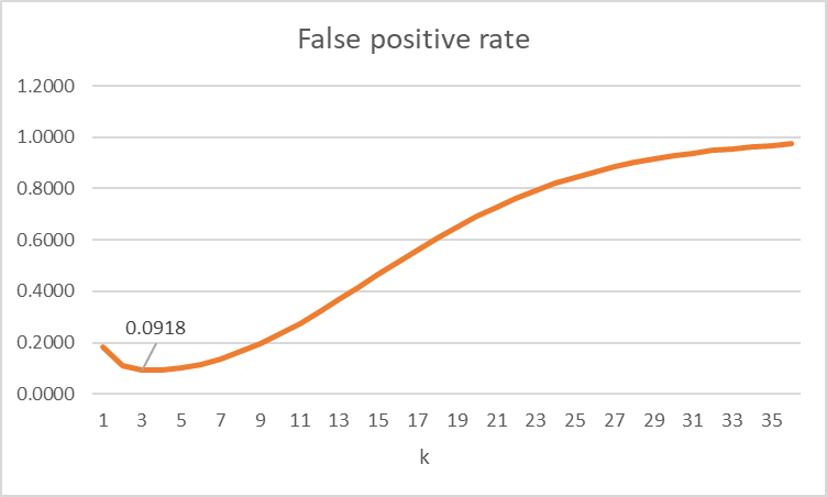
\includegraphics[width=0.8\textwidth]{./Figures/false_positive.png}\\	
	\caption{False positive rates}
	\end{figure}

	
	\section*{Exercise 3}
	
	The PageRank algorithm described in in Section 5.1 and 5.2
(Leskovec, Rajaraman and Ullman) has been implemented in Python. The script is saved in as the source file PageRank.py that is included in the assignment submission. 

	Our implementation primarily relied on the Python pandas library, particularly the data processing methods for dataframes. Most of the computation required for the algorithm was implemented as column operations on dataframes. 
	
	Firstly, the input file was written to a dataframe. The number of edges from each node was then calculated and stored in a separate dataframe. This was then merged back to the input dataframe as a new column, so that each FromNodeId had an associated number of edges. In another new column, 1 was divided by the number of edges, which allowed the non-zero elements of the transition matrix to be represented as a dataframe column. 
	
	A separate dataframe is used to represent the probability distribution of the location of a random surfer at each iteration of the algorithm. Probabilities are initialised to 1 divided by the number of nodes. Another merge operation is performed to create a new column in the main dataframe with the current probability distribution, again joining on the FromNodeId column. 
	
	By multiplying the transition probability with the current PageRank probability at each iteration, we can compute the individual products required for the dot products in matrix multiplication. The final dot products are computed by summing the individual products, having grouped by the ToNodeId column. 
	
	The top ten nodes by the largest PageRank have been included below. This result was obtained by running 60 iterations of the algorithm, at an execution time of 96.762 seconds. \\
	
	\begin{tabular}{cc}
	Node Id & PageRank \\
	\hline
  	41909 & 0.000439 \\
 	504140 & 0.000425 \\
 	597621 & 0.000416 \\
 	751384 & 0.000402 \\
 	486980 & 0.000402 \\
 	384666 & 0.000400 \\
 	537039 & 0.000394 \\
 	605856 & 0.000390 \\
  	32163 & 0.000384 \\
 	765334 & 0.000373 \\
	\hline 
	\end{tabular} \\\\

	\section*{Exercise 4}
	
	The following results were calculated using the Excel workbook that was included in the assignment submission. The $h(x)$ function was entered as a formula in the workbook, and the binary representation of this number of obtained using an inbuilt formula. The maximum tail length was observed in the binary numbers, which was then used to determine the estimate of the number of distinct elements. 
	
	\subsection*{Scenario 1}
	
	\subsubsection*{Question 1}
	
	The tail length for each stream element is calculated in the table below. The resulting estimate of the number of distinct elements in the stream is $2^{0}=1$. \\
	
	\begin{tabular}{cccc}
	$x$ & $h(x)$ & $h(x)$ binary & tail length \\
	\hline
	3 & 7 & 00111 & 0 \\
	1 & 3 & 00011 & 0 \\
	4 & 9 & 01001 & 0 \\
	6 & 13 & 01101 & 0 \\
	5 & 11 & 01011 & 0 \\
	9 & 19 & 10011 & 0 \\
	\hline
	\end{tabular}
	
	\subsubsection*{Question 2}
	
	The tail length for each stream element is calculated in the table below. The resulting estimate of the number of distinct elements in the stream is $2^{4}=16$.\\
	
	\begin{tabular}{cccc}
	$x$ & $h(x)$ & $h(x)$ binary & tail length \\
	\hline
	3 & 16 & 10000 & 4 \\
	1 & 10 & 01010 & 1 \\
	4 & 19 & 10011 & 0 \\
	6 & 25 & 11001 & 0 \\
	5 & 22 & 10110 & 1 \\
	9 & 2 & 00010 & 1 \\
	\hline
	\end{tabular}

	\subsubsection*{Question 3}
	
	The tail length for each stream element is calculated in the table below. The resulting estimate of the number of distinct elements in the stream is $2^{4}=16$.\\

	\begin{tabular}{cccc}
	$x$ & $h(x)$ & $h(x)$ binary & tail length \\
	\hline
	3 & 7 & 01100 & 2 \\
	1 & 3 & 00100 & 2 \\
	4 & 9 & 10000 & 4 \\
	6 & 13 & 11000 & 3 \\
	5 & 11 & 10100 & 2 \\
	9 & 19 & 00100 & 2 \\
	\hline
	\end{tabular}
	
	\subsection*{Scenario 2}	
	
	\subsubsection*{Question 4}
	
	The tail length for each stream element is calculated in the table below. The resulting estimate of the number of distinct elements in the stream is $2^{2}=4$. \\
	
	\begin{tabular}{cccc}
	$x$ & $h(x)$ & $h(x)$ binary & tail length \\
	\hline
	4 & 26 & 11010 & 1 \\
	5 & 0 & 00000 & 0 \\
	6 & 6 & 00110 & 1 \\
	7 & 12 & 01100 & 2 \\
	10 & 30 & 11110 & 1 \\
	15 & 28 & 11100 & 2 \\
	\hline
	\end{tabular}
	
	\subsubsection*{Question 5}
	
	The tail length for each stream element is calculated in the table below. The resulting estimate of the number of distinct elements in the stream is $2^{0}=1$.\\
	
	\begin{tabular}{cccc}
	$x$ & $h(x)$ & $h(x)$ binary & tail length \\
	\hline
	4 & 13 & 01101 & 0 \\
	5 & 15 & 01111 & 0 \\
	6 & 17 & 10001 & 0 \\
	7 & 19 & 10011 & 0 \\
	10 & 25 & 11001 & 0 \\
	15 & 3 & 00011 & 0 \\
	\hline
	\end{tabular}

	\subsubsection*{Question 6}
	
	The tail length for each stream element is calculated in the table below. The resulting estimate of the number of distinct elements in the stream is $2^{3}=8$.\\

	\begin{tabular}{cccc}
	$x$ & $h(x)$ & $h(x)$ binary & tail length \\
	\hline
	4 & 8 & 01000 & 3 \\
	5 & 10 & 01010 & 1 \\
	6 & 12 & 01100 & 2 \\
	7 & 14 & 01110 & 1 \\
	10 & 20 & 10100 & 2 \\
	15 & 30 & 11110 & 1 \\
	\hline
	\end{tabular}
	
	\newpage	
	
	\section*{Exercise 5}
	
	\subsection*{Part 1}
	
	This theory tells us about the locality and the sensitivity function which are very similar to locality hashing. The difference is people can use the other function to produce the pairs and also these functions which can apply to use the space sets or the other spaces and distance measure. For the functions they may have multiple conditions. One of these are having to collect the closest pairs to become the candidate pair because when we use the functions to consider two values are candidate pairs are not. Now we need to hash first two values of two values are equal then those pairs are candidate pairs. And if the two hashing values are not equal then the functions will determinate those two values are not candidate pair, If two hashing values are not equal then the functions are called family function.  For example family of hashing function and usually we use form(d1, d2,p1,p2) to expression of the locality function and d1 is smaller than d2. When these distances are bigger or may be equal d2 then x, y is a candidate pair. By the word, peoples don't have any kind of rule to determinate the distance between the d1 and d2 but we should let d1 and d2 be as close as possible, not when the distance between d1 and d2 is smaller then its a chance that p1 and p2 will be closet pair. The second condition is each and every pair must be independent of each other. The third condition is to be function will be highly efficient to determinate the candidate pair and reduce the false positive rate.
	
	The signal of the hashing function may not be fit for these conditions, so the minimum may be able to find the hash in the short time but signal hashing function is incompatible. If someone wants to find the family of locality sensitive function then they can only use the family of the min hashing function and assume that measured distance is Jaccard distance. We use the same way to summarise the min hash function, and then x and y will be candidate pairs, which is how we get the family of sensitive hash function. Hence it is proven that when Jaccard distance x and y will equal to the probability that a min hash function will have hash x and y  with same value. Thus, we can use the same way to find the d2.  In the locality of sensitive function we have two algorithms AND and OR construction to construct the family of sensitive function and the new can get the new family of function f. Each and every members of the function f is going to be produce by r members of function in F. Another construction is OR, here we can use OR construction to construct F. By these we can use AND construction and we will be reducing every probability.  

	\subsection*{Part 2}
	
	There are many ways to evaluate the similarities between these vectors. This summary is going to introduce the distance such as cosine distance and normal Euclidean distance which have some special ability to dictate locality sensitive families.
	
	\subsubsection*{LSH Families and Hamming distance}
	 
	There is a way of hamming distance to indicate the similarities into binary data strings where they have the same length and measuring methods to measure the hamming distance which is comparing how many different bit positions there are in two binary string. Like if someone wants to compare five with three with the use of hamming distance then first we are going to transfer both five and three to binary data, like 1010 and 1100 with due respect. Now we observe there  is a difference between 1010 and 1100 so the hamming distance between five and three is respectively 2. We go to know that if two binary data strings is completely same then their hamming distance will be 0 here the hamming distance is going to show does similarity of two data, which is based on the findings, here we are going to introduce hamming distance which is going to measure vector similarity. Here we know that the vector is a set of various types of numerical numbers, different dimensions is measured by different numbers so it is possible to randomly select position of any two vectors that we want to get compared and finding the hamming distance of the two vectors. Such as fi(x)=xi and fy(y)=yi. There is a law off hamming distance LSH. where we know that Jaccard distance will only runs on 0 to 1. when some vectors have very low dimensions show the result of similarities are not accurate.
	
	\subsubsection*{Hyperplanes and the Cosine Distance}

	As we all know hyperplanes are subspace of ambient space. Here the dimensions of hyperplane will be the dimensions of ambient space like assume that the ambient space have 3D space ,and the hyperplane of this ambient space 2d, here the space is 2D space, the hyperplane will be 1D line, because by the reduced dimension the hyperplane has infinite choice in lower dimensions.


\bibliography{./bibliography-ChapterSummary}
\end{document}
